In the previous chapter, we introduced our motivating scenario and the main ideas for answering the research questions. 
Based on this, the current chapter describes the setup of the experiments that are carried out in this thesis. %The following sections provide details of the experiments. 
Section~\ref{section:baseline} explains the baseline model that we use for all our experiments as an out-domain pre-trained model. Then, Section~\ref{section:datasets} provides the details of in-domain datasets and preprocessing steps applied to the datasets. Section~\ref{section:phrase_extraction} explains the process of extracting phrase pairs from the in-domain datasets. Finally, Section~\ref{section:fine-tuning} covers the details of fine-tuning processes. In particular, we show the several methods for presenting phrase pairs to the NMT model during fine-tuning.


\section{Baseline Model}\label{section:baseline}

We use the Transformer-based NMT system \parencite{vaswani2017attention} pre-trained by Facebook for the WMT'19 news translation task \parencite{ng-etal-2019-facebook}. It is released as part of the \textsc{Fairseq} toolkit \parencite{ott-etal-2019-fairseq}\footnote{\url{https://github.com/pytorch/fairseq}}. This model basically follows a big Transformer architecture from \cite{vaswani2017attention}, except using the larger feed-forward network (FFN) sub-layers size (8192). It was trained on Paracrawl 27.7M sentences, and was fine-tuned on several previous years WMT news-test sets for an additional epoch. Fairseq team released an ensemble of these four models but for our study we only use 'model 1'. 
%To simulate a realistic production setup, we start from a strong NMT sys- tem pre-trained on large amounts (28M sentences) of publicly available data.

Based on our scenario, to simulate a realistic production setup, a baseline model that has high performance for out-domain translation is required. This model satisfies this requirement: It was ranked first in the WMT'19 news competition \parencite{barrault-etal-2019-findings} with a BLEU score of 40.8 on a German-English news task. 


\section{Data}\label{section:datasets}
%why we chose public data instead of confidential data
%In the scenario (Section~\ref{section:scenario}), the original data is highly sensitive since it contains core information that the data owner wants to protect. 
We simulate the scenario of confidential data by using publicly available datasets in several technical domains: medicine descriptions, software manual and EU legislation. We consider these domains because they generally contain sensitive information that an adversary may abuse for profit or other reasons. 

%Short description of datasets
We evaluate our approach on a German to English translation task. For different technical domains, we choose EMEA (medical), GNOME (software) and JRC-Acquis (legal)~\parencite{steinberger2006jrc}. EMEA is a parallel text of medical guidelines from European Medicines Agency. GNOME is a collection of the text from GNOME desktop environment and software platform. JRC is a collection of legislative text from the European Union. All the public corpora are from the OPUS project \parencite[]{tiedemann-2012-parallel}\footnote{\url{https://opus.nlpl.eu/}}.%Note that, for avoiding confusion, we refer to JRC-Acquis as JRC in this paper. 

\subsection{Preprocessing}

For a realistic simulation of a professional translation scenario, we split the datasets by documents. This allows keeping track of the documents from which the sentences in the datasets were extracted. In future work, this could help the quantification of reconstructing the original documents from the extracted phrases.

All datasets are tokenized by \textsc{Moses Tokenizer} \parencite{koehn-etal-2007-moses}. To remove some defects from the parallel corpora that can affect the quality of NMT models, we filter out sentence pairs where either the source or target sentence is empty. We also remove duplicate sentences per documents. 

To segment our data, we use the same sub-word algorithms and split rules applied on the baseline model (Section \ref{section:baseline}) in \textsc{Fairseq} pipeline.
NMT has a fixed vocabulary size that can cause out-of-vocabulary (OOV) word issues. To mitigate this, \textsc{Fairseq} uses Byte Pair Encoding (BPE)~\parencite{sennrich-etal-2016-neural} for its subword segmentation algorithm. %that encodes words as sequences of sub-tokens, 
Especially, the baseline model used \textsc{FastBPE} implementation\footnote{\url{https://github.com/glample/fastBPE}} and we apply it to encode our data into sub-tokens.  
In addition, the baseline NMT model was pre-trained on a separate corpus, and the dictionary was built based on it. When fine-tuning on additional data, it is crucial to ensure that the new data gets consistent indices with the dictionary that it was originally trained on. Thus, we use the original dictionary from \textsc{Fairseq} for embedding our datasets. 

We assure that there is a limit to the possible amount of in-domain dataset. The original text of phrases that may be given to the translation company would still consist of quite small amount of sentences. Based on this, we reserve 10K sentence pairs and 2K sentence pairs for training and test set respectively. For early stopping (Section~\ref{chapter:early_stopping}), we reserve only 150 sentence pairs as a small validation set. The details of data statistics are shown in Table~\ref{tab:data_description}.
We release the benchmarks at \url{https://github.com/Sohyo/Using-Confidential-Data-for-NMT}.

%Using a document level data 
\begin{table}[ht]
\centering
\begin{tabular}{@{\ } ccccc @{\ }}
\Xhline{3\arrayrulewidth}
{Type}                   & {Domain} & Sentences               & Tokens (\textsc{de}) & Tokens (\textsc{en})     \\ \hline
\multirow{3}{*}{Train} & EMEA   & \multirow{3}{*}{10k} & 199k      & 209k          \\
                       & GNOME  &                      & 179k       & 194k \\
                       & JRC    &                      & 279k       & 396k          \\ \hline
\multirow{3}{*}{Validation}& EMEA   & \multirow{3}{*}{150} & 3k         & 3k            \\
                       & GNOME  &                      & 3k         & 3k             \\
                       & JRC    &                      & 4k         & 5k             \\ \hline
                      % 
\multirow{3}{*}{Test}  & EMEA   & \multirow{3}{*}{2k}  & 38k        & 42k            \\
                       & GNOME  &                      & 29k        & 30k        \\
                       & JRC    &                      & 53k        & 82k          \\ \Xhline{3\arrayrulewidth}
\end{tabular}
\caption{Details of datasets used in our fine-tuning experiments. The number of Tokens are round down to the nearest thousand.}
\label{tab:data_description}
\end{table}

\section{Phrase Extraction}\label{section:phrase_extraction}

%phrase extraction overview
In Chapter~\ref{chapter:methodology}, we suggest \textit{phrase extraction} as a text fragmentation technique in our experiments. It is a major element in the whole pipeline of Phrase-based SMT (PBSMT) model \parencite{koehn-etal-2003-statistical}. PBSMT uses phrase pairs obtained by using a word-aligned parallel corpus as base units in the translation model sub-component. For our experiments, only the phrase extraction step is used. Figure~\ref{fig:phrase_extraction} describes the steps of phrase extraction. 

We first word-align the in-domain datasets using \textsc{FastAlign}~\parencite{dyer-etal-2013-simple}\footnote{\url{https://github.com/clab/fast\_align}}, an unsupervised word aligner. In this step, the word aligner finds the best word alignments in two separate directions (source-to-target and target-to-source) and then combines them based on the symmetrization heuristics to obtain the alignment $A$~\parencite{och-etal-1999-improved, koehn-etal-2003-statistical}. In our experiments, we take the \textit{union} of the two alignments for the symmetrization $A$. Then we use the phrase extraction utility from the \textsc{Moses} phrase-based SMT toolkit \cite{koehn-etal-2007-moses}\footnote{\url{http://www.statmt.org/moses}} to extract all phrases consistent with $A$. After the phrase extraction step, our dataset has been fragmented into a list of aligned phrases of various lengths. An example of extracted phrase pairs is shown in Appendix~\ref{section:phrase_sample}.

A maximum source-side phrase length should be specified. 
We experiment with this number by setting the maximum phrase length to 1, 4 or 7. To prevent the full reconstruction of the original data by using the phrases, we randomly discard 50\% of the whole extracted phrases. Note that, because phrase pairs are considered as new parallel inputs for fine-tuning the NMT system, we extract phrases only from the training set.

%%%%%%%%%%%
%compute the union of source-to-target and target-to-source word alignment links (known as union symmetrization heuristic) to obtain the alignment $A$.
%If we simply form the intersection of the alignments, this will promote very precise alignments, but we will miss some of them. That’s why we do an intermediate thing and add alignment points from the union (growing the intersection).
%We use \textit{phrases} as a text fragmentation method which ensures data confidentiality while leaving the sentence alignment valid. Phrases are basically groups of words that are segmented from the input sentences. Phrase pairs are extracted using heuristic word-to-word alignment. As Figure \ref{fig:example_phrase} illustrates, the words of the target language(German) are aligned with the words of the source language(English). Based on this, the phrases are statistically translated into target language and reordered. In this paper we will often mention using only phrases smaller than a certain length, here we only restrict the target phrase length. For instance, in Figure \ref{fig:example_phrase}, the green boxes represent a phrase of length two: 'der Nachrichtenlist' is the German phrase and 'the list of messages' is the English phrase. In our experiments, the goal is to find the optimal way in which to represent the extracted phrases to pre-trained NMT model.

\begin{figure}[h]
    \centering
    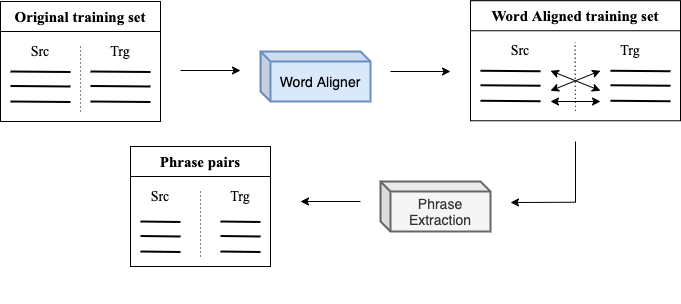
\includegraphics[scale=0.46]{images/phrase_extraction.png}
    \caption{Process of phrase extraction.}
    \label{fig:phrase_extraction}
\end{figure}

\section{Fine-tuning}\label{section:fine-tuning}

%fine-tuning steps : details / phrase datasets
%In Section~\ref{section:pipeline}, we represent the pipeline of our experiments and for both methods, we use fine-tuning. 
%Finetuning refers to continuing to train a pre-trained model on a training set within a domain. 
In Section~\ref{section:pipeline}, we showed the two pipelines of our experiments consisting of the standard and proposed method, respectively. Both methods use fine-tuning, which indicates continuing to train the pre-trained model on an in-domain training set.

To establish an upper bound of the translation quality of domain adaptation, we first conduct the standard method, a common fine-tuning technique for domain adaptation. To do so, we fine-tune the baseline model on full sentences of the original in-domain datasets. 
%For the proposed method, however, the full sentences of the in-domain data are not fed into the NMT system. 
On the other hand, during fine-tuning for the proposed method, we provide phrase pairs to the models as if they were sentence pairs. After the phrase extraction step, the in-domain phrase datasets has many duplicates.
Finally, to study the utility of the phrase pairs, we experiment with various setups for the fine-tuning process. 
%and this will be covered in Section~\ref{section:experiments}

% In this work, we focus on how to effectively use phrases for fine-tuning. %Our main idea is to fine-tune different lengths of phrases to examine the usefulness of them and see if this could benefit more from tagging technique. 
% The main point of our research is to examine the effect of using phrases with different maximum lengths on the fine-tuned models' performance. Furthermore we aim to find out how different phrase lengths interact with our tagging technique.
% %Based on this, we experiment different ways to sub-sample the set of pairs used for fine-tuning.

\subsection{Varying maximum phrase lengths}

To explore the difference in the efficiency of phrases of different length, we fine-tune by using various maximum phrase lengths. Although the sentence structure or context information is all broken, we conjecture the NMT model can learn new terminology from fine-tuning on maximum length 1, equivalent to a dictionary of the in-domain dataset. The longer the phrase (max lengths 4 and 7), the richer the amount of in-domain information for domain adaptation the phrase is expected to hold.

\subsection{Tagging}

As explained in Section~\ref{section:tagging}, we hypothesise that a tagging technique on phrases can prevent the short output bias in phrase-adapted NMT models.
%Phrase pairs differ from the full sentences that the baseline model previously trained on and training NMT models on such short segments can cause a bias that generates shorter output translation. We hypothesise that a tagging technique \parencite{sennrich2016controlling} can prevent this bias in our NMT models. 
We experiment with a simple tagging technique by adding <PT> and </PT> at the front and end of each phrase respectively, in both source and target side. During testing, full sentences with no tags are given to the model. Table~\ref{tab:tagged_phrase_example} shows an example of a source-target pair of full sentences and a pair of phrases with tags from the EMEA dataset. 
%For instance, consider the following German-English phrases pair:\\

\begin{table}[hb!]
\centering
\begin{tabular}{P{0.145\linewidth}| P{0.03\linewidth}| p{0.75\linewidth}}
\Xhline{3\arrayrulewidth}
 & De &
  In den meisten Fällen wird der Serumferritinwert simultan zum Anstieg des \textcolor{blue}{Hämatokritwertes abfallen} . \\ \cline{2-3}
\multirow{-2}{*}{\textbf{Sentence}} &
  En &
  In most cases , the ferritin values in the serum fall simultaneously with the rise in \textcolor{blue}{packed cell volume} .
 \\ \hline\hline
                              & De & {<PT> Hämatokritwertes abfallen </PT>} \\ \cline{2-3}
\multirow{-2}{*}{\textbf{Phrase $+$tags}} & En & <PT> packed cell volume </PT>                             \\ \Xhline{3\arrayrulewidth}
\end{tabular}
\caption{A sample of a pair of full sentences and a phrase pair with tags. The phrases are extracted from the given sentences.}
\label{tab:tagged_phrase_example}
\end{table}

% \begin{table}[hb]
% \centering
% \begin{tabular}{P{0.03\linewidth}| p{0.9\linewidth}}
% \Xhline{3\arrayrulewidth}
% \multicolumn{2}{c}{\textbf{Original sentence}}                                                                      \\ \hline\hline
% \multicolumn{1}{c|}{\textbf{De}} &
%   In den meisten Fällen wird der Serumferritinwert simultan zum Anstieg des \textcolor{blue}{Hämatokritwertes abfallen} \\ 
% \multicolumn{1}{c|}{\textbf{En}} &
%   In most cases , the ferritin values in the serum fall simultaneously with the rise in \textcolor{blue}{packed cell volume} . \\ \hline
% \multicolumn{2}{c}{\textbf{Phrases with tags}}                                                                      \\ \hline\hline
% \multicolumn{1}{c|}{\textbf{De}} & <PT> Hämatokritwertes abfallen </PT> \\ 
% \multicolumn{1}{c|}{\textbf{En}} & <PT> packed cell volume </PT>        \\ \Xhline{3\arrayrulewidth}
% \end{tabular}
% \caption{A sample of a pair of full sentences and a phrase pair with tags. The phrases are extracted from the given sentences.}
% \label{tab:tagged_phrase_example}
% \end{table}

\subsection{Fine-tuning Hyperparameters}

We apply the hyper-parameters described by \cite{ng-etal-2019-facebook} with only a few adjustments inspired from previous work on fine-tuning regularization~\parencite{miceli-barone-etal-2017-regularization}. Specifically, the learning rate is divided by 4 (0.000175) and  for early stopping, we use a small (full-sentence) validation set in each domain (150 sentences, see Table~\ref{tab:data_description}). We set the weight decay rate to 0.0001 and dropout probability to 0.2 after varying experiments. All details of other parameters of the fine-tuning are described in Table~\ref{tab:hyperparameter}.
%only alter the learning rate to 4 times smaller (0.000175). 
%In addition, fine-tuning large NMT models on relatively small in-domain datasets for domain adaptation can be difficult due to a risk of overfitting. 
%To prevent overfitting, we use several techniques: early stopping, drop out \cite{srivastava2014dropout} and weight decay. Especially, \cite{miceli-barone-etal-2017-regularization} reported that early stopping can prevent overfitting, even though it requires held-out training dataset (validation dataset). We fine-tuned several times to discover the optimal setup for each of the full sentences and phrases in each domain. After varying experiments, we set the weight decay rate as 0.0001 and dropout probability as 0.2. 
%We evaluate the quality of NMT models by BLEU score (Section~\ref{section:evaluation_metrics}). To compute this, we use \textsc{SacreBLEU}~\parencite{post-2018-call}.\footnote{\url{ https://github.com/mjpost/sacrebleu}}
We run all the experiments on a node with a \textsc{NVIDIA} V100 GPU in the Peregrine high-performance computing (HPC) cluster of the University of Groningen.\footnote{\url{https://portal.hpc.rug.nl/public/start.html}}


\begin{table}[ht!]
\centering
\begin{tabular}{c|c}
\Xhline{3\arrayrulewidth}
\textbf{Hyperparameter}             & \textbf{Value} \\ \hline
Maximum number of tokens in a batch & 4096 tokens    \\ \hline
Optimizer                           & Adam           \\ \hline
Learning rate                       & 0.00017        \\ \hline
Epoch                               & 20             \\ \hline
Best checkpoint metric              & BLEU           \\ \hline
Beam search size                    & 5              \\ \hline
Drop out                            & 0.2            \\ \hline
Weight decay                        & 0.0001         \\ \hline
Label smoothing                     & 0.1            \\ \Xhline{3\arrayrulewidth}
\end{tabular}
\caption{Hyperparameters for all fine-tuning Transformer based baseline (Section~\ref{section:baseline}) experiments.}
\label{tab:hyperparameter}
\end{table}